\documentclass[11pt]{article}

\usepackage[T1]{fontenc}
\usepackage[utf8]{inputenc}
\usepackage{lmodern}
\usepackage[margin=1in]{geometry}
\usepackage{microtype}
\usepackage{amsmath,amssymb}
\usepackage{booktabs}
\usepackage{tabularx}
\usepackage{longtable}
\usepackage{makecell}
\usepackage{multirow}
\usepackage{array}
\usepackage{enumitem}
\usepackage{xcolor}
\usepackage{caption}
\usepackage{algorithm}
\usepackage[noend]{algpseudocode}
\usepackage{listings}
\usepackage{tikz}
\usetikzlibrary{arrows.meta,positioning,fit,calc}
\usepackage[numbers,sort&compress]{natbib}
\usepackage[colorlinks=true,linkcolor=black,citecolor=blue!50!black,urlcolor=blue!50!black]{hyperref}

\newcommand{\prim}[1]{\textmd{\textsc{#1}}}
\newcolumntype{Y}{>{\raggedright\arraybackslash}X}
\setlist{nosep,leftmargin=*}
\setlist[description]{font=\normalfont\bfseries,style=nextline,labelindent=0pt}
\captionsetup{font=small,labelfont=bf}

\title{\textbf{Agent = Harness(Model):}\\Five Mechanistic Primitives, and What Is Not One}
\author{Chase Dovey\\Average Joes Lab\\\texttt{https://cdovey.dev}}
\date{}

\begin{document}
\maketitle

\begin{abstract}
The software around a language model in an agent is called a scaffold, a framework, a runtime or a harness, and none of these names comes with a definition of what the thing contains. We take the position that an LLM agent is a model wrapped in a harness, $\textit{Agent} = \textit{Harness}(\textit{Model})$, and that every harness is built from five mechanistic primitives: \prim{Input}, which captures what comes in; \prim{Context}, which assembles what the model is shown; \prim{Model interface}, which sends the request and brings back the response; \prim{Output}, which carries the response out; and \prim{Control flow}, which decides whether to go again, hand back or stop. Each primitive is defined by what it does and by what it never does, so that the five are mutually exclusive. We then separate three levels at which harnesses can be described: the \emph{primitives}, which every harness has; the \emph{design decisions} made within each primitive, which is where harnesses differ; and the \emph{production concerns} (persistence, safety and security, observability, resilience, performance, evaluation), which are questions asked of every primitive rather than parts of the harness. As evidence, we deconstruct six harnesses from their primary sources at pinned versions: Claude Code, Codex CLI, opencode, pi, Hermes Agent, and a LangGraph workflow. Every component we found has a home in one primitive or one concern, and the differences between the six are design decisions within the primitives. The vocabulary gives a procedure for locating an agent's failure in one of five places before attributing it to the model, and a schema for reporting the harness alongside the model. The minimal harnesses from which the definitions were drawn are reproduced in an appendix, and the evidence for every assignment is published with the paper.
\end{abstract}

\section{The Architecture}
\label{sec:architecture}

A language model is a function from a sequence of tokens to a distribution over the next token, applied until a stop token is produced:
\[
  \textit{TokensOut} = \textit{Model}(\textit{TokensIn}).
\]
Viewed from outside, the model keeps no state between calls, cannot read from or act on its environment, and cannot call itself again. Chat templates, tool-call formats and reasoning tokens are conventions for laying out \textit{TokensIn} and reading \textit{TokensOut}; models learn them in training and can learn to emit calls to tools \citep{schick2023toolformer}, but the calls are carried out, and the conventions written and parsed, by something else.

That something else is the harness: everything in an agent that is not the model. It turns the world into tokens for the model and the model's tokens into effects on the world.
\[
  \textit{Agent} = \textit{Harness}(\textit{Model}).
\]
The boundary is at the model's weights and its sampling. Memory across sessions, tool use and knowledge of the date or the working directory are all on the harness side. The software has many names: evaluations call it a \emph{scaffold} \citep{anthropic2025swebench,metr2025update}, libraries call themselves \emph{frameworks}, \emph{SDKs} or an \emph{orchestration framework and runtime} \citep{langgraph}, and \emph{harness} is common among people who build coding agents \citep{anthropic2025harnesses}. None of the names says what the thing contains.

We propose that it contains five parts, and that the five are the same in every harness.

\begin{description}
  \item[\prim{Input}] captures what comes in.
  \item[\prim{Context}] assembles what the model is shown.
  \item[\prim{Model interface}] sends the request and returns the response.
  \item[\prim{Output}] carries the response out: words to a person, actions on the world.
  \item[\prim{Control flow}] decides whether to go again, hand back, or stop.
\end{description}

Figure~\ref{fig:loop} shows how they sit around the model, and Algorithm~\ref{alg:harness} gives the loop they form, each line labelled with its primitive. Something comes in: a request from a person, an event, or the result of an earlier action. The harness assembles a context around it and sends the context to the model. The harness handles the response: it shows words to a person, or carries out the actions the response requests. If an action produced a result, the result comes back in and the loop runs again; if not, control returns to the person, or the agent stops. Every harness in \S\ref{sec:deconstruction} is an elaboration of this loop.

\begin{figure}[t]
\centering
\resizebox{\linewidth}{!}{%
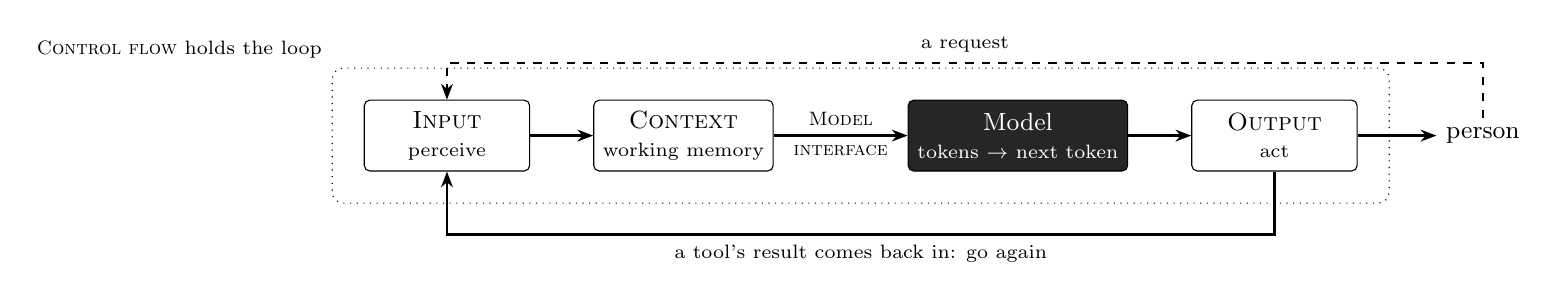
\begin{tikzpicture}[
  node distance=8mm and 8mm,
  box/.style={draw, rounded corners=2pt, minimum width=21mm, minimum height=9mm, align=center, font=\small},
  model/.style={box, fill=black!85, text=white, minimum width=27mm},
  arr/.style={-{Stealth[length=2mm]}, thick}]
  \node[box] (in) {\prim{Input}\\[-1pt]\scriptsize perceive};
  \node[box, right=of in] (ctx) {\prim{Context}\\[-1pt]\scriptsize working memory};
  \node[model, right=17mm of ctx] (m) {Model\\[-1pt]\scriptsize tokens $\to$ next token};
  \node[box, right=of m] (out) {\prim{Output}\\[-1pt]\scriptsize act};
  \node[font=\small, right=10mm of out] (p) {person};
  \draw[arr] (in) -- (ctx);
  \draw[arr] (ctx) -- node[above, font=\scriptsize]{\prim{Model}} node[below, font=\scriptsize]{\prim{interface}} (m);
  \draw[arr] (m) -- (out);
  \draw[arr] (out) -- (p);
  \draw[arr] (out.south) -- ++(0,-8mm) -| node[pos=0.25, below, font=\scriptsize]{a tool's result comes back in: go again} (in.south);
  \draw[arr, dashed] (p.north) -- ++(0,7mm) -| node[pos=0.25, above, font=\scriptsize]{a request} (in.north);
  \node[draw, dotted, rounded corners=4pt, inner sep=4mm, fit=(in)(ctx)(m)(out), label={[font=\scriptsize]north west:\prim{Control flow} holds the loop}] {};
\end{tikzpicture}}
\caption{The agent loop. The five primitives surround the model; \prim{Control flow} decides whether the loop runs again, hands back, or stops.}
\label{fig:loop}
\end{figure}

\begin{algorithm}[t]
\caption{A harness. Lines are labelled with the primitive they implement.}
\label{alg:harness}
\small
\begin{algorithmic}[1]
\Procedure{ControlFlow}{\,}
  \State $\textit{conversation} \gets [\,]$
  \Loop \Comment{outer loop: one request at a time}
    \State $\textit{conversation}.\textsc{append}(\textsc{User}(\Call{Input}{\,}))$ \Comment{\prim{Input}: from a person}
    \Loop \Comment{inner loop: one request, carried through}
      \State $\textit{ctx} \gets \Call{Context}{\textit{conversation}}$ \Comment{\prim{Context}}
      \State $\textit{response} \gets \Call{ModelInterface}{\textit{ctx}}$ \Comment{\prim{Model interface}}
      \State $\textit{conversation}.\textsc{append}(\textsc{Assistant}(\textit{response}))$
      \State $\textit{results} \gets \Call{Output}{\textit{response}}$ \Comment{\prim{Output}: show words, run actions}
      \If{$\textit{results} = \emptyset$} \textbf{break} \Comment{nothing ran: hand back}
      \EndIf
      \State $\textit{conversation}.\textsc{append}(\textsc{User}(\textit{results}))$ \Comment{\prim{Input}: from the world}
    \EndLoop
  \EndLoop
\EndProcedure
\end{algorithmic}
\end{algorithm}

Everything else said about a harness is at one of two other levels. A \emph{design decision} is one way of implementing a primitive: one tool or forty, a loop or a graph, a repository map or a summarizer. A \emph{production concern} is a question asked of every primitive: what should outlast the session, what could do harm, what did it do, what if something breaks, what is slow, how do we know it still works. Neither adds a primitive (\S\ref{sec:levels}).

\paragraph{Scope.} The primitives describe what happens on the path of a request at run time. Software that ships with a harness but never acts on that path is out of scope: hosting and transport, configuration loading, packaging, the user-interface framework, and the infrastructure that carries telemetry. The model is held fixed. A program that makes one model call and prints the reply has a harness, a trivial one; what makes a harness an agent's is a \prim{Control flow} that feeds the results of actions back to the model.

\paragraph{What this paper does.} \S\ref{sec:primitives} shows each primitive as the smallest program that adds it. \S\ref{sec:levels} separates the primitives from design decisions and production concerns. \S\ref{sec:vocabulary} says why a shared vocabulary for the harness is needed and what it is for: comparing primitives by their implementations, and isolating a failure to the primitives an implementation touches. \S\ref{sec:deconstruction} deconstructs the popular harnesses against the five: six from their sources at pinned versions, and a wider set from their sources or documentation at summary level. \S\ref{sec:further} sets out the comparisons that would both use the framework and test it. The minimal harnesses are in Appendix~\ref{app:minimal}, the rules for the cases at the boundaries in Appendix~\ref{app:rules}, and the evidence for every assignment in Appendix~\ref{app:evidence}.

\section{The Five Primitives}
\label{sec:primitives}

Algorithm~\ref{alg:harness} gives a harness as pseudocode, each line labelled with its primitive. Every harness in \S\ref{sec:deconstruction} is an elaboration of it. For each primitive we give its \emph{mechanism} (what it does on the path of a request), its \emph{negative definition} (what it never does, and which primitive does), and its \emph{design space} (the decisions a harness makes within it). The negative definitions make the five mutually exclusive: each piece of a harness has one home, assigned by its function rather than by its name or its location in the code.

\begin{algorithm}[t]
\caption{A harness. Lines are labelled with the primitive they implement.}
\label{alg:harness}
\small
\begin{algorithmic}[1]
\Procedure{ControlFlow}{\,}
  \State $\textit{conversation} \gets [\,]$
  \Loop \Comment{outer loop: one request at a time}
    \State $\textit{conversation}.\textsc{append}(\textsc{User}(\Call{Input}{\,}))$ \Comment{\prim{Input}: from a person}
    \Loop \Comment{inner loop: one request, carried through}
      \State $\textit{ctx} \gets \Call{Context}{\textit{conversation}}$ \Comment{\prim{Context}}
      \State $\textit{response} \gets \Call{ModelInterface}{\textit{ctx}}$ \Comment{\prim{Model interface}}
      \State $\textit{conversation}.\textsc{append}(\textsc{Assistant}(\textit{response}))$
      \State $\textit{results} \gets \Call{Output}{\textit{response}}$ \Comment{\prim{Output}: show words, run actions}
      \If{$\textit{results} = \emptyset$} \textbf{break} \Comment{nothing ran: hand back}
      \EndIf
      \State $\textit{conversation}.\textsc{append}(\textsc{User}(\textit{results}))$ \Comment{\prim{Input}: from the world}
    \EndLoop
  \EndLoop
\EndProcedure
\end{algorithmic}
\end{algorithm}

\subsection{\prim{Input}: capture what comes in}
\textbf{Mechanism.} Capture what enters the agent and hand it to \prim{Context}. There are two sources: a person (a message, a file, an interrupt, an answer to a question the model asked) and the world (the result of an action, an event, a scheduled trigger).
\textbf{Never.} \prim{Input} never decides what the model is shown; that is \prim{Context}. It never runs anything; that is \prim{Output}. An answer a person gives that the \emph{harness} consumes, such as an approval, is not input but a \prim{Control flow} decision; an answer the \emph{model} consumes, returned as a tool result, is input.
\textbf{Design space.} The source: a terminal, an editor, a chat channel, a command-line argument, an issue tracker, a webhook, a message queue. The kind: text, images, files, audio, the results of actions, interrupts, and mid-turn steering. The second source, results from the world, is what makes acting worthwhile: an action's result is new perception.

\subsection{\prim{Context}: assemble what the model is shown}
\textbf{Mechanism.} Assemble, for one call, everything the model is shown: instructions, the tools' descriptions, the conversation so far, and anything retrieved from memory or the environment; and fit it to the window, by truncation, compaction or selection. \prim{Context} is the agent's working memory, rebuilt on every call.
\textbf{Never.} \prim{Context} never calls the model; that is \prim{Model interface}. It never acts on the world; that is \prim{Output}. Reading a memory store is \prim{Context}; writing one, if the model requests it, is an action and so \prim{Output}. Code that decides what the model sees is \prim{Context} even when it sits inside a tool: a tool that attaches project instructions to a file it reads, or condenses a web page before returning it, is doing \prim{Context}'s work.
\textbf{Design space.} What goes in the instructions (identity, rules, the agent's own capabilities, project files such as \texttt{AGENTS.md}); how tools are described; how long-term memory comes in (preloaded, retrieved on demand, or searched by the agent through its own tools); the roles each piece is placed in, which carry authority; and what happens when the window fills: drop old turns, summarize them, or include only what the moment needs.

\subsection{\prim{Model interface}: reach the model}
\textbf{Mechanism.} Send the assembled context to the model and bring back its response in a form the rest of the harness can read: words, and structured requests to act. This includes the client, the wire format, the translation between the harness's message format and the model's chat template, streaming, retrying a failed request, and switching to a backup model when the request could not be served.
\textbf{Never.} \prim{Model interface} never decides what the request contains; that is \prim{Context}. It never acts on the response; that is \prim{Output}. It receives a stream; rendering each fragment as it arrives is \prim{Output}. A change of model because the request could not be served (unavailable, overloaded, refused) is \prim{Model interface}; a change of model keyed to the work (planning, a cheap model for a side task) is \prim{Control flow}.
\textbf{Design space.} A hosted API or local inference; one provider or many, directly or through a translation layer; native tool-call formats or tool calls parsed from text; streaming or whole responses; retry policy and backup models. \prim{Model interface} is the only primitive that knows which model is inside, which is why changing the model means changing it alone.

\subsection{\prim{Output}: carry the response out}
\textbf{Mechanism.} Handle what the model returned: show its words to a person, and carry out each requested action, collecting its result. The tool set, the executor that runs an action, and the environment it runs in are \prim{Output}.
\textbf{Never.} \prim{Output} never decides whether to go again; that is \prim{Control flow}. It never assembles the next request; that is \prim{Context}. The model only ever \emph{requests} an action; \prim{Output} decides whether and how it happens, which is where sandboxes and never-lists live. Several tool calls from one response run concurrently: \prim{Output}. Several \emph{model} calls run concurrently: \prim{Control flow}. A program the model writes at run time that calls tools without calling the model is \prim{Output}; one that sequences model calls is \prim{Control flow}.
\textbf{Design space.} The tool set, from one general tool (a shell) to dozens of specific ones (read, write, edit, search, browse, computer use); the action format, from structured tool calls to code the model writes and the harness executes \citep{wang2024codeact} to edit formats such as search-and-replace blocks; the execution environment, from the host machine to a container or a remote sandbox; and the presentation of results, including truncation and error messages, which \citet{yang2024sweagent} show affect performance.

\subsection{\prim{Control flow}: decide what happens next}
\textbf{Mechanism.} Define the shape of the loop: send results back and go again, hand back to the person, or stop. Step and token budgets, approval gates the harness consumes, delegation to sub-agents and the sequencing of several agents, and routing to a model keyed to the work are all \prim{Control flow}.
\textbf{Never.} \prim{Control flow} never captures input, assembles context, calls the model or runs a tool. It sequences the other four. A workflow in which code fixes the order of model calls \citep{anthropic2024effective} and an agent in which the model directs its own process differ here and only here.
\textbf{Design space.} A single open loop that runs until the model stops requesting actions; a fixed pipeline; an explicit graph; sub-agents with contexts of their own; planning or approval modes that change what is allowed; and stopping rules: step limits, budgets, interrupts, loop detection.

\subsection{Necessity}
Each primitive answers a question no other answers: what comes in, what the model is shown, how the model is reached, what is done with what comes out, and what happens next. Appendix~\ref{app:minimal} gives the five minimal harnesses from which the definitions were drawn, built one primitive at a time around a fixed model and task. Each version fails in a specific way without the next primitive: with only \prim{Model interface}, the model answers but cannot act and nobody can ask it anything else; with \prim{Input}, anyone can ask and it still cannot act; with \prim{Output}, it acts once and the result goes nowhere; with \prim{Control flow}, it finishes the task but does not know what it is or where it is, and spends actions finding out; with \prim{Context}, it knows. This shows that each primitive removes a failure the others do not. It does not show that no sixth primitive could ever be needed; \S\ref{sec:deconstruction} tests that against existing harnesses, and \S\ref{sec:limitations} says what would refute it.

\section{Design Decisions and Production Concerns}
\label{sec:levels}

Descriptions of harnesses mix three kinds of statement. ``It has a loop'' names a primitive. ``It gives the model forty tools'' names a decision within one. ``It runs commands in a sandbox'' names a measure taken for a reason that applies to every primitive. Keeping the three apart is the main use of the vocabulary. A primitive is a mechanism every harness has, defined by its function on the request path; a harness has exactly five. The other two levels are where harnesses differ and where they are made fit to run.

\subsection{Design decisions}
A design decision is one way of implementing a primitive. It is the level at which harnesses differ, and the level at which they are usually described. A design decision never adds a primitive; it fills one. The test for whether something is a design decision is whether a different harness could make a different choice and still be a harness. Table~\ref{tab:decisions} lists the decisions found in the deconstruction of \S\ref{sec:deconstruction}, by primitive, with the choices the harnesses made.

\begin{table}[t]
\centering
\small
\setlength{\tabcolsep}{4pt}
\caption{Design decisions by primitive, and the choices seen across the harnesses deconstructed in \S\ref{sec:deconstruction}.}
\label{tab:decisions}
\begin{tabularx}{\linewidth}{@{}l>{\raggedright\arraybackslash}p{3.1cm}Y@{}}
\toprule
Primitive & Decision & Choices seen \\
\midrule
\prim{Input} & source & terminal; editor; chat gateways; HTTP; issue tracker; scheduled trigger; a typed state channel \\
 & mid-turn messages & delivered at the next step boundary (steer); after the turn (queue); as an interrupt; not at all \\
 & the person's answers & consumed by the harness as approvals; returned to the model as tool results \\
\addlinespace
\prim{Context} & instructions & a system prompt alone; plus project files (\texttt{CLAUDE.md}, \texttt{AGENTS.md}); plus memory files; a sectioned prompt diffed into patches \\
 & long-term memory & none; files preloaded into the instructions; a store searched by the agent through tools; summaries carried forward \\
 & window fitting & drop old turns; summarize (prune, then summarize); compaction at a threshold with a verbatim tail; provider-native compaction; left to user code \\
 & layout for caching & a stable prefix with changes appended; instruction changes frozen as dated events; byte-stable tiers \\
\addlinespace
\prim{Model interface} & client & provider SDK; in-house request compiled per protocol; one stream function over adapters; a library's chat-model call \\
 & transport & HTTP with server-sent events; WebSocket, falling back to HTTP \\
 & retries and backup & none; three to ten retries; retry split by whether output started; a fallback chain of models \\
 & action format & native tool calls; calls parsed from text; a code block to execute \\
\addlinespace
\prim{Output} & tool set & one shell; a fixed built-in set; built-in plus MCP; plain tool objects; a tool node \\
 & action format & structured calls; model-written code run in an interpreter (V8, QuickJS, in-process) \\
 & execution environment & the host; an OS sandbox with a domain allowlist; a container; a remote sandbox \\
 & parallelism & sequential; read-only calls concurrent; all calls concurrent as they stream \\
\addlinespace
\prim{Control flow} & loop shape & until no tool call; one task per turn; a user-written graph run as supersteps; a phase-verdict loop \\
 & stopping rules & step budget; token or cost budget; unlimited; recursion limit; stop-gate nudges \\
 & approval & a rule pipeline ending in a prompt; a classifier model; a reviewer model; each tool asserting its own permission \\
 & delegation & an agent tool to a fixed depth; child sessions; sub-agents as full sessions; flat threaded delegation \\
\bottomrule
\end{tabularx}
\end{table}

\subsection{Production concerns}
A production concern is a question asked of every primitive, whose answer changes how some primitives are implemented. We use six (Table~\ref{tab:concerns}): what should outlast the session (persistence); what could do harm, and who could make it (safety and security); what did it do (observability); what if something breaks (resilience); what is slow or costly (performance); and how do we know it still works (evaluation). A concern is not a part of the harness. A sandbox is not a sixth primitive; it is the safety answer in \prim{Output}. A memory store is not a sixth primitive; it is a store in the world that \prim{Context} reads and \prim{Output} writes, kept for the persistence concern. A trace is not a sixth primitive; it is the observability answer, recorded wherever the primitive it watches runs. The test for whether something is a concern is whether it is motivated by a question that could equally be asked of a different primitive.

\begin{table}[t]
\centering
\scriptsize
\setlength{\tabcolsep}{3pt}
\caption{Six production concerns as questions asked of each primitive. Each cell names what the concern changes in that primitive; ``---'' means we found nothing essential there in the harnesses examined.}
\label{tab:concerns}
\begin{tabularx}{\linewidth}{@{}l*{6}{Y}@{}}
\toprule
& \textbf{Persistence} & \textbf{Safety \& security} & \textbf{Observability} & \textbf{Resilience} & \textbf{Performance} & \textbf{Evaluation} \\
& \emph{What outlasts the session?} & \emph{What could do harm, and who could make it?} & \emph{What did it do?} & \emph{What if something breaks?} & \emph{What is slow or costly?} & \emph{Does it still work?} \\
\midrule
\prim{Input} & an unfinished session offered back & approvals asked of a person & refusals recorded & input ending; interrupts & --- & yes to every approval in a test run \\
\prim{Context} & memories; resumed transcripts & untrusted content; poisoned memory; roles and authority & --- & compaction when too long & caching the unchanged prefix; trimming results & the instructions under test \\
\prim{Model interface} & --- & --- & tokens, latency, cost per call & retries; a backup model & streaming & the model under test \\
\prim{Output} & --- & sandboxes; never-lists; secrets hidden; pinned images & what each action did & time limits on actions & parallel actions; smaller models for side tasks & the tools under test \\
\prim{Control flow} & the task in progress; a diary of every message & runaway loops; the record kept out of reach & each decision & resume after a crash & --- & the loop under test \\
\bottomrule
\end{tabularx}
\end{table}

The concerns interact. Persistence creates a security surface: a poisoned memory steers every later session. Streaming changes safety: an interrupt can stop a reply mid-sentence, and the harness must record what was said rather than a finished answer. Summarizing changes persistence: the summary must say where the originals are kept. Treating concerns as questions asked of each primitive makes these interactions visible; treating them as separate components hides them.

\subsection{Bundles and the cases at the boundaries}
Much of what a harness's documentation names is a bundle. A mode, a skill, a hook system or an agent profile packages decisions across several primitives: a planning mode is a context template, a restricted tool set and an approval gate; a hook system is a dispatcher in \prim{Control flow} whose events each affect one primitive. Decomposed, each element has one home. The negative definitions decide most placements. Thirteen rules, each needed for a component found in \S\ref{sec:deconstruction}, decide the rest, and are given in Appendix~\ref{app:rules}. Three are used often enough to state here. A component is assigned by its function, not its location: an approval decision made inside a tool's runtime is \prim{Control flow}. A sub-agent is a harness of its own, and delegation to it is \prim{Control flow} of the outer harness. And one primitive may use another's mechanism to do its job: \prim{Context} may ask the model to summarize old turns before compacting them, and the component is assigned by what it decides, with the call it makes a use of \prim{Model interface}.

\section{Why a Vocabulary}
\label{sec:vocabulary}

\subsection{Harnesses change results as much as models do}
If $\textit{Agent} = \textit{Harness}(\textit{Model})$, a benchmark score belongs to the pair. The evidence that the harness term is large is now direct. Holding GPT-4 Turbo fixed, \citet{yang2024sweagent} report 1.31\% of SWE-bench \citep{jimenez2024swebench} resolved with retrieval-augmented generation and 12.47\% with their agent, and on SWE-bench Lite 11.00\% for a shell-only agent against 18.00\% for SWE-agent, with only the harness changing. Anthropic notes that performance ``can vary significantly based on this scaffolding, even when using the same underlying AI model'' \citep{anthropic2025swebench}. METR found that tailoring a scaffold to one model more than doubled the length of tasks it could complete \citep{metr2025update}, and later that two mature harnesses did not outperform their default scaffolds \citep{metr2026harness}, which suggests the effect is largest where the design decisions differ most. \citet{zhang2026stop} argue that harness configuration can account for more variance in performance than the choice of model, and ask that the harness be disclosed when agents are compared; \citet{kapoor2025hal} evaluate models, scaffolds and benchmarks as separate dimensions.

A disclosure needs a schema, and a comparison needs the harness stated in parts. Without one, two agents built on the same model are compared as wholes, and a difference between them cannot be attributed to anything smaller than ``the scaffold''. The five primitives are the schema: the input sources; what the context holds and how it is fitted to the window; the provider, decoding settings and retry policy; the tools, their output formats and the execution environment; and the loop's shape and stopping rules. Table~\ref{tab:summary} and Table~\ref{tab:wide} are such disclosures for nineteen harnesses.

\subsection{Comparing primitives by their implementations}
With the harness stated in five parts, a question that could not be asked becomes well-posed: which implementation of a primitive is better, for which model, on which task? The form of the study is to hold the model and four primitives fixed, vary the fifth, and measure. \citet{fan2026empirical} do this for three decisions in a coding harness, planning, the action space and context management, across four models, and find that each changes behaviour. Their three dimensions were chosen independently of this paper and each falls within one primitive: planning in \prim{Control flow}, the action space in \prim{Output}, context management in \prim{Context}. The vocabulary says what the other dimensions are, and says which parts must be held fixed for a result to be attributed to the one varied. \S\ref{sec:further} lists the comparisons the framework makes well-posed.

The same property makes a harness portable. Because only \prim{Model interface} knows which model is inside, a harness can be moved to a new model or provider by changing that primitive alone. A harness loses this property when model-specific details leak into other primitives: a provider's tool-call format assumed in \prim{Output}, or a provider's error strings matched in \prim{Context} management. The deconstruction records such leaks where it found them. It also says what a model trained for one harness must learn: the context layout it will be shown (\prim{Context}), the format in which it must request actions and the shape of the results it will read (\prim{Output}), and the loop it runs in (\prim{Control flow}).\footnote{In the companion book, a 0.6-billion-parameter model instruction-tuned on sessions recorded in its own harness rose from 2 to 18 of 32 held-out tasks in that harness, where the same base model post-trained by its developers for general use scored 14. The experiment, its data and its checks are described there \citep{course}; this paper makes no claim that rests on it.}

\subsection{Isolating a failure}
\label{sec:debugging}
When an agent fails, the primitives give a short list of places to look, in order. The order matters: each question rules out a place the next question assumes.
\begin{enumerate}
  \item \textbf{\prim{Context}: was the model shown what it needed?} Read the request that was sent. If the file, the result or the instruction is not in it, the model could not have used it, and nothing downstream is at fault.
  \item \textbf{\prim{Output}: did what it asked for happen?} Compare the action the model requested with what ran. A parser that dropped a call, a sandbox that refused it, a tool that returned a truncated result, and an error message the model could not read are all \prim{Output}.
  \item \textbf{\prim{Control flow}: did the loop stop early or run too long?} A step limit reached before the task was done, a hand-back on a response that still had work in it, and a loop that repeated the same action are \prim{Control flow}.
  \item \textbf{\prim{Model interface}: was the response read correctly?} A tool call emitted in the right format but not recognized, a stream cut off and treated as complete, and a backup model substituted without notice are \prim{Model interface}.
  \item \textbf{\prim{Input}: did the right thing come in?} A result delivered to the wrong turn, an interrupt lost, a person's answer consumed by the harness when the model needed it.
  \item \textbf{Only then, the model.} If the model was shown what it needed, asked for the wrong thing, and its request was carried out as asked, the failure is the model's: its knowledge, its habits, or its size.
\end{enumerate}
An implementation touches some primitives and not others, and a failure is isolated to the ones it touches. Two examples from our own transcripts. A small model, after instruction-tuning, sometimes emitted a second tool call as bare JSON without its \texttt{<tool\_call>} tags. The harness read the JSON as words, found no action, and handed back. Question 4 locates this in \prim{Model interface}, whose parser defines what counts as a call; the fix was on the model side, but the diagnosis was the harness's. In the same experiments, four kinds of task could never pass during reinforcement learning because the check compared the folder before and after, and the harness's own memory directory changed the folder on every run. No question in the list locates this, because the fault was in the evaluation, a concern, not in a primitive. Building the harness around a capable model first, until it passed every task in the evaluation, is what let every later failure be attributed to the model swapped in.

\subsection{Existing vocabularies}
\label{sec:related}
The loop that harnesses implement goes back to ReAct \citep{yao2023react}, which interleaves a model's reasoning with actions whose results return to it as observations; in artificial intelligence more broadly, an agent perceives its environment and acts on it \citep{russell2020aima}. Later patterns live in particular primitives: Reflexion \citep{shinn2023reflexion} writes reflections on failed attempts and carries them into the next, a decision in \prim{Control flow} and \prim{Context}; MemGPT \citep{packer2023memgpt} pages information in and out of a limited window, a decision in \prim{Context}; Toolformer \citep{schick2023toolformer} trains the model to emit tool calls, moving policy into the model while the calls are still carried out by \prim{Output}; CodeAct \citep{wang2024codeact} has the model write code as its action format, a decision in \prim{Output}.

\citet{sumers2024coala} organize language agents by memory (working, episodic, semantic, procedural), an action space of external and internal actions, and a decision cycle. CoALA describes what an agent \emph{is}, as a cognitive architecture; this paper describes what software an agent is \emph{made of}. The correspondence is in Table~\ref{tab:coala}. Two things here have no counterpart there: \prim{Model interface} as a component, and the production concerns as a level of description distinct from the architecture. CoALA's memory modules, with the retrieval and learning actions that read and write them, are design decisions in \prim{Context} and \prim{Output} here, not a component.

\begin{table}[t]
\centering
\small
\caption{The five primitives, the step of the agent cycle each serves, and the CoALA component it corresponds to.}
\label{tab:coala}
\begin{tabularx}{\linewidth}{@{}lYYY@{}}
\toprule
Primitive & Mechanism & In the agent cycle & CoALA \\
\midrule
\prim{Input} & capture requests and results & perceive & observations \\
\prim{Context} & assemble what the model is shown & working and long-term memory & working memory; retrieval \\
\prim{Model interface} & request a response & decide & reasoning (by the model) \\
\prim{Output} & show words, carry out actions & act & grounding actions; learning (writes) \\
\prim{Control flow} & go again, hand back, or stop & the cycle & decision cycle \\
\bottomrule
\end{tabularx}
\end{table}

\citet{yang2024sweagent} name the agent-computer interface, the commands a model is given, their output format and guardrails such as linting edits, and show it changes performance on software tasks; in our terms the interface is a set of design decisions in \prim{Output} and \prim{Context}, and this paper asks what the complete set of components is, of which the interface is part. \citet{anthropic2024effective} distinguish workflows, in which code fixes the sequence of model calls, from agents, in which the model directs its own process, and describe patterns built on an ``augmented LLM''; we treat the distinction as a property of \prim{Control flow}, and decompose the augmented LLM into \prim{Context} (retrieval, memory) and \prim{Output} (tools) around a \prim{Model interface}. \citet{jin2026agentprimitives} use ``primitives'' for recurring patterns of model calls in multi-agent systems (review, voting, planning and execution); in our terms these are shapes of \prim{Control flow}, and the two uses of the word are complementary. Tool protocols such as MCP \citep{mcp} provide pluggable \prim{Output}, with their other features assigned by function (Appendix~\ref{app:rules}).

\section{Deconstruction}
\label{sec:deconstruction}

If the architecture holds, a harness built by someone else, for a different purpose, at a different scale, should decompose into the five primitives with nothing left over, and its differences from other harnesses should be locatable as design decisions within a primitive. We test this on the popular harnesses, in two sets.

\paragraph{Selection.} The first set is six harnesses in wide use whose primary sources were available, read in depth: two command-line coding agents from model developers (Claude Code \citep{claudecode} and Codex CLI \citep{codexcli}), two open-source coding agents built outside the model developers (opencode \citep{opencode} and pi \citep{pi}), one general-purpose agent built for messaging platforms as well as the terminal (Hermes Agent \citep{hermes}), and one workflow framework (LangGraph \citep{langgraph}), for which we deconstruct the canonical agent it ships, a ReAct loop, together with the runtime that executes it. The workflow framework tests the claim that a workflow and an agent differ only in \prim{Control flow}. The second set is thirteen more, read at summary level: the coding agents SWE-agent, OpenHands, Aider, Cline, Gemini CLI and Goose, the agent frameworks OpenAI Agents SDK, Google ADK, AutoGen, CrewAI and smolagents, and two closed harnesses read from their documentation alone, Cursor and GitHub Copilot's coding agent. Claude Code is likewise deconstructed from its documentation, since its source is not published. The nineteen are the harnesses we could read, not a sample of all harnesses; \S\ref{sec:notshown} says what that leaves untested.

\paragraph{Method.} For each harness we (i) read the source at a pinned commit, or the documentation on a stated date, and mapped the path of a request from the moment a message arrives to the next model call; (ii) assigned every component on that path to exactly one primitive, or to one production concern together with the primitive it changes, by the definitions of \S\ref{sec:primitives} and the rules of Appendix~\ref{app:rules}, citing a file and line range or a page and section for each; and (iii) recorded every component that was hard to place and how it was resolved, or that it was not. For the first set every component on the path was assigned; for the second, two to five components per primitive, chosen as the ones that define the harness's design decision there. Components outside the request path (hosting, packaging, UI frameworks) were noted and left unassigned. The evidence is in Appendix~\ref{app:evidence} and in the repository as a file per harness; the subsections below summarize the first set.

%% PER-HARNESS SUBSECTIONS: filled from the evidence files
\subsection{Claude Code}
Anthropic's coding harness, deconstructed from its documentation as read on 15 October 2026 \citep{claudecode}; its source is not published. The loop is the open one of Algorithm~\ref{alg:harness}: the model is called until it returns a response with no tool calls, and a turn's result carries why it ended (done, a turn limit, a cost budget, an error). \prim{Input} has one entry point for everything that starts a turn: typed prompts, piped input, messages queued mid-turn and delivered after the current tool batch, scheduled prompts, and reports from background sub-agents. \prim{Context} is built as a stable cached prefix (the system prompt, the tools, then project files such as \texttt{CLAUDE.md}) with later updates appended as messages or system reminders; tool schemas for MCP servers are deferred behind a search tool; and compaction, on reaching the window, is a separate request that re-injects the project files, memory, recently read files and invoked skills. \prim{Model interface} is the Messages API with streaming, up to ten retries that never re-issue after a completed tool block, idle watchdogs, and a fallback chain the user configures. \prim{Output} is a fixed built-in tool set plus MCP tools; read-only calls run concurrently and mutating calls in sequence; shell commands run under an OS sandbox with a domain-allowlist proxy; large results spill to files; file edits are checkpointed for rewind. \prim{Control flow} adds a six-step permission pipeline (hooks, deny rules, ask rules, the permission mode, allow rules, then a prompt), delegation through an agent tool to a depth of three, and, at scale, a model-written JavaScript workflow the runtime executes, which sequences model calls and is therefore \prim{Control flow} by the rule on model-written programs.

Three components were hard to place. The web-fetch tool calls the model itself to condense a page before the main model sees it: the call is \prim{Output}, the condensing is a \prim{Context} decision, and the extra request is \prim{Model interface}. The default permission gate in ``auto'' mode is a second model asked to classify each action: a \prim{Control flow} gate implemented as a model call with its own stripped context. And a server-side variant of that classifier runs inside the API during the session's own requests, so the harness only consumes its verdict; we return to this in \S\ref{sec:summary}.

\subsection{Codex CLI}
OpenAI's terminal and IDE coding agent, at commit \texttt{f0c5077} \citep{codexcli}, written in Rust. A session is one thread that receives typed operations over a channel; a dispatcher matches each one (a turn's input, an interrupt, an approval, the answer to a question, a compaction request) and runs each user turn as a task. \prim{Input} is that channel: text typed during a running turn is queued as steering rather than starting a new turn, an inter-agent mailbox and asynchronous hook results merge into the same pending-input queue, and the model's questions to the person come back as a typed answer. \prim{Context} is the Responses API's own item list, with the environment and instructions injected as typed ``world-state'' sections sent as diffs when they change, project files walked from the root to the working directory, and tool outputs truncated in the live history only; compaction has three implementations (a local summary, a remote one performed by the server, and a token-budget reset), chosen by explicit threshold arithmetic, and can run speculatively in the background once usage passes a percentage of the window. \prim{Model interface} is the Responses API only, WebSocket first with a session-wide fallback to HTTP, five retries with jittered backoff that honour the server's retry timing, an idle timeout, and requests sent without server-side storage, with encrypted reasoning replayed. \prim{Output} routes every risky action through one orchestrator (approval, then the platform sandbox, then the run, then a retry if the sandbox denied it), with Seatbelt on macOS, seccomp with bubblewrap and Landlock on Linux and a restricted token on Windows; tools run concurrently under a read--write gate that lets parallel-safe tools overlap; and a ``code mode'' runs model-written JavaScript in V8, each nested tool call re-entering the harness's approval and sandbox path. \prim{Control flow} is one task per turn, looping until the model emits no tool call, with stop hooks, roll-over into compaction mid-turn, an approval precedence of hooks, then an optional model reviewer (``Guardian''), then the person, and sub-agents that are full sessions of their own with depth and thread caps.

Hard cases: the Guardian is a \prim{Control flow} gate whose verdict comes from a nested harness; the remote compaction is a \prim{Context} decision whose summarizer is the provider; over WebSocket the request omits the tools and instructions the server already holds, so what is sent depends on transport state while what the model is shown does not; and the plan-mode parser, which reads the streamed text into a proposed-plan item and can redirect it, is \prim{Output} rendering that also feeds the stop decision. We record the last as straddling \prim{Output} and \prim{Control flow} by design.


\subsection{opencode}
An open-source coding harness by Anomaly, at commit \texttt{654b79b} \citep{opencode}; it was rewritten since earlier versions, and the deconstruction describes the current one. Each session is an event-sourced record in SQLite, and one fibre per session drains a durable inbox: \prim{Input} is a row in that inbox, from a person, a shell command, a skill, or the harness itself, marked for delivery either at the next step boundary (``steer'') or after the current turn (``queue''). \prim{Context} re-projects the event history into model messages on every call, with instructions placed in a cached prefix and changes to them frozen into the history as dated events; compaction is triggered at about ninety percent of the window, using provider-measured token counts plus a local estimate, keeps the newest fifteen thousand tokens verbatim, and can be delegated to the provider's native compaction. \prim{Model interface} is an in-house request type compiled per provider protocol (Anthropic Messages, OpenAI Responses, Bedrock Converse, Gemini), streamed over HTTP or a stateful WebSocket, with a retry policy split by whether output had already started. \prim{Output} runs tool calls concurrently as they stream, and most tools are reachable only through one \texttt{execute} tool that runs model-written JavaScript in an interpreter that cannot call the model, which the rule on model-written programs places in \prim{Output}. \prim{Control flow} continues while a step made tool calls, stops on a text-only finish, enforces an optional per-agent step budget, and delegates to child sessions (depth one by default), whose results return as tool text or as a synthetic message.

Hard cases: every tool asserts its own permission, so an approval gate the harness consumes lives inside the tool's code (\prim{Control flow} by function); the step budget is enforced by appending an assistant message and disabling tools, a \prim{Control flow} decision carried out by editing what the model sees; and the compaction service both decides what to summarize and issues the model call itself. Native provider-side compaction leaves the harness's \prim{Context} holding an item it cannot inspect.

\subsection{pi}
A terminal coding agent by Mario Zechner, at commit \texttt{5ab7fe7} \citep{pi}, built in layers: a minimal agent loop, a provider layer, and a coding-agent session on top. \prim{Input} comes from a terminal editor, a print mode, or a JSON-RPC mode, all into one \texttt{prompt()} call, with mid-run messages split into steering (after this turn) and follow-ups (after the agent would have stopped). \prim{Context} is a projection of a persisted session tree: a compaction entry, the kept tail, and context edits, with the system prompt kept as named sections and diffed into patches, so that replaying the file reproduces the exact request; compaction triggers when the context exceeds the window less a reserve, and keeps the most recent twenty thousand tokens. \prim{Model interface} is one streaming function behind about fifteen provider adapters, with the SDKs' own retries disabled so that the harness owns a two-tier retry policy, and an overflow classifier that routes a too-long request to compaction rather than to a retry. \prim{Output} is a set of plain tool objects run in parallel by default, with mutations to one file serialized; there is no sandbox in the core (OS sandboxing and permission prompts are extensions), and a ``code mode'' tool runs model-written scripts in a QuickJS sandbox. \prim{Control flow} is a two-level loop (tool calls and steering inside, follow-ups outside) plus a session-level loop for retries, overflow recovery and extension continuations; sub-agents are not in the core, though an example spawns child processes; and per-request routing between ``virtual models'' is keyed to the reason for the request.

Hard cases: a wire-level hook lets an extension rewrite the request body, which is \prim{Context} by function though it sits in the adapter; the virtual-model router has a ``retry'' branch that overlaps the backup-model rule (we place it in \prim{Control flow}, since the router decides by the state of the work); and the code-mode script can call auxiliary models from inside the sandbox, a model call issued from inside a tool, which we discuss in \S\ref{sec:summary}. A telemetry interface exists, but no span is emitted at this commit.

\subsection{Hermes Agent}
A personal agent by Nous Research, at commit \texttt{7bf3766} \citep{hermes}, with one agent core behind a terminal interface, about twenty-five messaging-platform adapters, an HTTP server, an ACP adapter and a cron scheduler. \prim{Input} is one normalized message event shared by all of these; mid-turn messages become steering rather than new turns. \prim{Context} is a three-tier system prompt, kept byte-stable so that caching holds: identity, then project files (capped by size), then volatile memory, skills and the time; compaction at half the window prunes, then summarizes with an auxiliary model; oversized tool output is spilled to files rather than dropped; and a tool-search bridge lets the model fetch tool schemas on demand. \prim{Model interface} is an OpenAI-style chat-completions client by default with pluggable transports for Anthropic, Responses and Bedrock, streaming on, three retries with backoff, then a configurable fallback chain, then a bounded auto-recovery wait. \prim{Output} sends a fixed core tool set on every call, splits each batch into parallel-safe segments, runs terminal commands behind pluggable sandboxes (local, Docker, Modal, and others) and a regex-plus-human approval gate, and persists each tool-call row before executing it. \prim{Control flow} is a loop of named phases, each returning a verdict, with an unlimited iteration budget by default, ``stop-gate'' nudges that append a synthetic message and go again, flat delegation to threaded children, and task-keyed routing to auxiliary models.

Two components do not fit cleanly. In one mode the whole turn is handed to an external Codex process, and Hermes keeps only input, persistence and a fallback: the five primitives collapse into one opaque external harness that is neither a sub-agent (there is no outer loop) nor the model. And ``providers'' reached over ACP make the thing behind the \prim{Model interface} another agent. Both are nested harnesses by the rule of \S\ref{sec:rules}, but of an unusual shape: the nesting is at the \prim{Model interface}, not in \prim{Control flow}.

\subsection{A LangGraph workflow}
LangGraph \citep{langgraph}, at commit \texttt{5eb60ae}, is a framework for writing control flow as a graph over a checkpointed state, executed by a runtime in bulk-synchronous supersteps. We deconstruct the agent it ships, \texttt{create\_react\_agent}, together with that runtime. \prim{Input} is a write to a named channel of a typed state, merged by a user-chosen reducer, whether it is a person's message, a tool result, or a resume value after an interrupt. \prim{Context} is exactly the state's message list, optionally prefixed by one system message; fitting it to the window is left entirely to a user-written hook before the model call, and the framework provides only a primitive for removing messages. \prim{Model interface} is one call to a LangChain chat model per step, and the framework contains no client of its own, no streaming of its own, and no backup model; retries and timeouts are per-node policies, off by default. \prim{Output} is a tool node that runs every tool call of a response concurrently in-process, turns results and (configurably) errors into messages, and lets a tool return a routing command. \prim{Control flow} is the graph: ``go again'' is a conditional edge from the agent node to the tool node and back, ``stop'' is an empty task set or a recursion limit, and a pause is an exception the runtime persists as a checkpoint write and resumes by re-running the node.

This is the clearest case of the three-level distinction. The framework fixes the five primitives' mechanisms and leaves most of the design decisions to user code: the edges, the stopping rule, the window-fitting hook, the approval gate around an interrupt, dynamic model selection, retry policies. A workflow and an agent built with it differ in the graph, which is \prim{Control flow}, and nowhere else. The hard cases are the step counter injected into the state (it looks like \prim{Context} but no model sees it; it is a \prim{Control flow} budget), and a scheduling packet that carries a state snapshot to the tool task (\prim{Control flow} carrying \prim{Context}).


\subsection{Summary}
\label{sec:summary}
Table~\ref{tab:summary} gives the six side by side, one row per primitive, and Table~\ref{tab:wide} the thirteen of the second set. Every component we found has a home. The differences between the harnesses are in the rows: what comes in and from where, what the context holds and how it is fitted, how the model is reached, which tools exist and where they run, and what shape the loop has. None of the nineteen required a sixth row.

\begin{table}[p]
\centering
\scriptsize
\setlength{\tabcolsep}{3pt}
\renewcommand{\arraystretch}{1.2}
\caption{Six harnesses by primitive. Each cell is the design decision that harness made within the primitive; the evidence for each is in Appendix~\ref{app:evidence}.}
\label{tab:summary}
\begin{tabularx}{\linewidth}{@{}>{\bfseries}p{1.9cm}YYYYYY@{}}
\toprule
& Claude Code & Codex CLI & opencode & pi & Hermes Agent & LangGraph \\
\midrule
\prim{Input} &
prompts, stdin, queued mid-turn messages, scheduled prompts, sub-agent reports, tool results, answers to an ask-user tool &
one operation channel per thread; steering queued mid-turn; mailbox; typed answers to the model's questions; tool results
 &
durable inbox rows (person, shell, skill, synthetic), delivered as steer or queue at step boundaries &
terminal, print and RPC modes into one prompt call; steer and follow-up queues &
one message event from CLI, 25 messaging gateways, HTTP, ACP, cron; mid-turn steering &
writes to a typed state channel, merged by a reducer: messages, tool results, resume values \\
\addlinespace
\prim{Context} &
cached prefix (system, tools, CLAUDE.md) plus appended reminders; deferred MCP schemas; compaction re-injects memory and recent files &
the Responses item list; world-state sections as diffs; project files walked to cwd; three compaction modes, with background compaction
 &
event-sourced history re-projected per call; cached instructions as dated events; compaction at $\sim$90\%, 15k tail, or provider-native &
projection of a session tree; sectioned prompt diffed into patches; compaction past a reserve, 20k tail &
three-tier byte-stable prompt; memory and project files; compaction at 50\% by prune then summarize; tool-search bridge &
the state's messages plus one system message; window-fitting left to a user hook \\
\addlinespace
\prim{Model}\newline\prim{interface} &
Messages API, streaming; 10 retries; idle watchdogs; user-configured fallback chain &
Responses API only; WebSocket, falling back to HTTP; 5 retries with server-advised timing; no server-side storage
 &
in-house request compiled per protocol; SSE or WebSocket; retry split by whether output started &
one stream function over $\sim$15 adapters; SDK retries off; two-tier retry; overflow routed to compaction &
chat-completions client with pluggable transports; streaming; 3 retries, fallback chain, auto-recovery &
one LangChain chat-model call per step; no client, streaming or fallback of its own \\
\addlinespace
\prim{Output} &
built-in tools plus MCP; read-only calls concurrent; OS sandbox with domain allowlist; results spill to files; edit checkpoints &
one orchestrator: approve, sandbox, run, retry on denial; OS sandboxes on three platforms; read--write gate for parallel tools; V8 code mode
 &
tools run concurrently as they stream; each asserts its own permission; most reached through a code-mode interpreter &
plain tool objects, parallel by default; no core sandbox; QuickJS code mode &
core tools plus bridge; parallel-safe segments; sandboxed terminal (local, Docker, Modal, \ldots); approval gate &
tool node runs calls concurrently in-process; errors become messages; tools may return routing commands \\
\addlinespace
\prim{Control flow} &
loop until no tool calls; six-step permission gate, with a classifier model by default; agent tool to depth 3; model-written workflows &
task per turn; loop until no tool call; hooks, Guardian reviewer, then person; sub-agents as full sessions with depth caps
 &
one fibre per session; continue while tools called; per-agent step budget; child sessions, depth 1 &
inner tool loop, outer follow-up loop, session loop for retries; virtual-model routing &
phase-verdict loop; unlimited budget; stop-gate nudges; flat threaded delegation; task-keyed routing &
a user-written graph run as supersteps; stop on empty task set or recursion limit; interrupts checkpointed \\
\bottomrule
\end{tabularx}
\end{table}

%% Placeholder until the wide-set evidence files are in: regenerated by evidence/wide_table.py
\begin{table}[p]
\centering
\scriptsize
\caption{Thirteen more harnesses by primitive, from their sources or documentation at summary level; the evidence for each cell is in Appendix~\ref{app:evidence}.}
\label{tab:wide}
(pending)
\end{table}


\paragraph{What was hard to place.} The hard cases are collected in Appendix~\ref{app:evidence}, and four recur across the first set.
\begin{itemize}
  \item \textbf{Primitives that call the model.} In Claude Code, opencode and pi, compaction decides what to summarize and then calls the model to summarize it; Claude Code's web-fetch tool and pi's code mode call models from inside a tool. Read as a call graph, these break the rule that \prim{Context} and \prim{Output} never call the model. Read as responsibility, they do not: the component still decides one thing, and uses \prim{Model interface} to do it. We added the rule on primitives as services (Appendix~\ref{app:rules}) for these cases.
  \item \textbf{Approval gates inside tools.} In opencode and Hermes the code that asks the person sits inside the tool that would act, and in Codex the approval requirement depends on what the sandbox allows. By function the gate is \prim{Control flow} and the enforcement is \prim{Output}; by location they are one file. The two also read each other, which is the interaction of concerns noted in \S\ref{sec:levels}.
  \item \textbf{Decisions carried out by editing the context.} opencode enforces a step budget by appending an assistant message and disabling tools; Hermes's stop gates append a synthetic message and go again; LangGraph replaces the model's answer with a canned message when the step budget is reached. Each is a \prim{Control flow} decision whose mechanism is a change to what the model is shown. The decision and the mechanism have different homes, and we record both.
  \item \textbf{Nesting at the model interface.} Hermes can hand a whole turn to an external Codex process, or reach an agent over ACP as if it were a model. The thing behind \prim{Model interface} is then another harness. The nested-harness rule covers it, but the nesting is at a different primitive from the sub-agent case, and the outer harness keeps only \prim{Input}, persistence and a fallback.
\end{itemize}
One finding is not a hard case but a boundary question. Claude Code's server-side classifier runs inside the API during the session's own requests, and opencode can delegate compaction to the provider. In both, a function the vocabulary places in the harness runs on the provider's side of the API, and the local harness holds only a verdict or an opaque item. The primitives still apply: the harness is split across two machines, not reduced to four parts. But it means the boundary of \S\ref{sec:architecture} is at the model's weights, not at the API, and a deconstruction from a client's source alone will miss the part that runs behind the API. We found no component in the nineteen that satisfied none of the five definitions.

\subsection{What the deconstruction does not show}
\label{sec:notshown}
\paragraph{Selection.} Nineteen harnesses, most of them coding agents or frameworks used for coding examples. Harnesses for browsing, voice, robotics and customer service were not examined, and the design decisions in Table~\ref{tab:decisions} are drawn from what these nineteen do. The selection criterion was wide use and the availability of sources; it is not a random sample.
\paragraph{Documentation-only analysis.} Claude Code, Cursor and Copilot are deconstructed from documentation, which states what the harness does but not always how. Negative definitions are harder to confirm from documentation than from source, and a documented feature may differ from the shipped one.
\paragraph{The harness is not always in one place.} Two of the six run part of their harness behind the provider's API. A deconstruction from client source or documentation describes the local part; the part on the provider's side is visible only through its effects. As providers absorb more harness functions, this gap will grow.
\paragraph{Products change.} Every assignment is pinned to a commit or a documentation date. Several of these harnesses change weekly. The deconstruction describes them on those dates, and a reader checking it later should use the pinned versions.
\paragraph{Who made the assignments.} The assignments were made by the author with an AI coding agent as a research instrument (see the disclosure), and each cites its evidence. No second, independent decomposition was made; \S\ref{sec:further} returns to this. The rules in Appendix~\ref{app:rules} are where disagreement would most likely arise: they follow from the definitions, but another reader could draw some boundaries elsewhere.
\paragraph{Coverage is not comparison.} That every component has a home shows the five cover what exists. It does not show that any implementation is better than another, which is the subject of \S\ref{sec:further}.

\section{Further Work: Comparing Implementations of a Primitive}
\label{sec:further}

The deconstruction shows that the five primitives cover what exists: every component in nineteen harnesses had a home in one primitive or one concern. It does not show which implementation of a primitive is better, for which model, on which task. That is the comparison the vocabulary makes well-posed, and it has not been done.

\paragraph{The form of the study.} Hold the model fixed. Hold four primitives fixed. Vary the fifth, one design decision at a time, and measure on a task set with a check that does not depend on the primitive varied. The harness is stated in the five parts of Table~\ref{tab:primitives}, so that the varied part is the only difference between arms, and the statement is published with the result. \citet{fan2026empirical} is the nearest existing study, with three decisions varied across four models; the vocabulary names the remaining decisions and says what must be held fixed.

\paragraph{One comparison per primitive.} The decisions in Table~\ref{tab:decisions} are the candidates. Within \prim{Context}: window fitting, where the harnesses in \S\ref{sec:deconstruction} drop old turns, summarize, compact at a threshold with a verbatim tail, or leave it to the provider, and no two agree on when; and the placement of project instructions, preloaded or searched. Within \prim{Output}: the action format, structured calls against model-written code run in an interpreter, which some of the nineteen offer and the rest do not; and the execution environment, host, OS sandbox or container, which changes what the model is allowed to do and what it is told it did. Within \prim{Control flow}: the stopping rule, a step budget against a cost budget against none; and the approval gate, a rule pipeline against a classifier model against per-tool assertion, measured on both task completion and the rate of harmful actions. Within \prim{Model interface}: the retry and backup policy, measured under induced provider failure. Within \prim{Input}: the delivery of mid-turn messages, at the next step boundary or after the turn, measured on tasks where the person changes the request part-way.

\paragraph{What such a study needs.} A task set with a harness-independent check. A model held at a fixed version, since the harness that suits one model may not suit another \citep{metr2025update}. The four fixed primitives reported in the same five-part schema, so that a later study can hold the same things fixed. And the evidence files of Appendix~\ref{app:evidence} are a starting point for the arms: each cell of Table~\ref{tab:summary} is an implementation that exists and can be ported into a common harness, because the primitives give the seam along which to port it.

\paragraph{These comparisons are also the test of the framework.} The deconstruction tests coverage: can every component be placed? A comparison tests something the deconstruction cannot: can a result be attributed to the primitive varied? If an implementation cannot be placed in one primitive, or if varying one primitive changes behaviour only through another, the framework is wrong in a way that reading source could not show. The five questions of \S\ref{sec:debugging} make the same prediction in the small: a failure isolated to one primitive should be fixed by a change to that primitive alone. Both predictions are checkable, and neither has been checked at scale.

\paragraph{A second coding of the deconstruction.} The assignments in Appendix~\ref{app:evidence} were made by the author with an AI coding agent as a research instrument, against the definitions of \S\ref{sec:primitives} and the rules of Appendix~\ref{app:rules}. No independent second coding was made, so the agreement between two people applying the definitions is unmeasured. The brief, the definitions and the component lists are published for that purpose.

\section{Conclusion}
\label{sec:conclusion}

We have argued that every LLM agent is a model wrapped in a harness, and that every harness is built from five primitives: \prim{Input}, \prim{Context}, \prim{Model interface}, \prim{Output} and \prim{Control flow}. The production concerns that make a harness safe and dependable are questions asked of these primitives, not additional parts. The harnesses in wide use today, however different they appear, make different decisions within the same five primitives.

The harness is where most of an agent's behaviour is decided: what it knows about itself and its situation, what it is able and allowed to do, how it recovers from failure, and when it goes again. It deserves to be named, decomposed and reported with the same care as the model inside it. We hope the vocabulary proposed here helps make that routine.

\section*{Disclosure of AI use}

AI tools were used in two roles.

\textbf{As a research instrument.} The deconstruction of \S\ref{sec:deconstruction} was carried out with an AI coding agent (Claude, Anthropic) under the author's direction. The agent read each harness's source at the pinned commit, or its documentation on the stated date, applied the definitions of \S\ref{sec:primitives} and the rules of Appendix~\ref{app:rules}, and recorded every assignment with a file-and-line or URL citation. The author reviewed the assignments and the hard cases. Every assignment in Appendix~\ref{app:evidence} can be checked against its cited source without the agent.

\textbf{As a writing assistant.} The author set the position, the structure, the definitions and the three-level vocabulary, and reviewed every section. An AI assistant drafted prose from the author's outline and notes, and edited for consistency. The minimal harnesses of \S\ref{sec:primitives} and Appendix~\ref{app:minimal}, and the transcripts they quote, are the author's.


\bibliographystyle{plainnat}
\bibliography{references}

\appendix
\section{The Minimal Harnesses, One Primitive at a Time}
\label{app:minimal}

The definitions in \S\ref{sec:primitives} were drawn from five programs, each the previous one plus one primitive, all run on the same task: a two-file Python project whose \texttt{total()} subtracts a discount as a flat amount where the test expects a percentage, and the request \emph{``The tests are failing. Find out why and fix it.''} The model is Claude Sonnet through Anthropic's Messages API; the files are \texttt{harness/1\_model\_interface.py} to \texttt{harness/quark.py} in the companion repository \citep{course}, reproduced here without their dependency headers. The transcripts quoted are from the recorded runs there. In the transcripts, \texttt{>} is what the person typed, \texttt{<} what the model said, and \texttt{\$} a command it ran.

\lstset{basicstyle=\ttfamily\scriptsize, columns=fullflexible, keepspaces=true, breaklines=true, frame=single, rulecolor=\color{black!25}, commentstyle=\color{black!55}, language=Python, showstringspaces=false}

\subsection{\prim{Model interface} alone}
\lstinputlisting[firstline=4]{minimal/1_model_interface.py}
The model answers, but it can only answer: \emph{``I don't have access to your code, test files, or test output. Nothing came through in your message besides the request.''} The request is written into the program, so nobody can ask it anything else. What is missing is a way for something to come in.

\subsection{Plus \prim{Input}}
\lstinputlisting[firstline=4,linerange={11-16}]{minimal/2_input.py}
Anyone can now type the request, and the answer is the same: \emph{``I don't have the code or the test output yet, so I can't tell why the tests are failing. Could you share\ldots''} It can only talk. What is missing is a way to act.

\subsection{Plus \prim{Output}}
\lstinputlisting[firstline=4,linerange={6-26}]{minimal/3_output.py}
A tool is described to the model, and \texttt{handle\_output} runs each command the model asks for and collects the result:
\begin{verbatim}
> The tests are failing. Find out why and fix it.
< I'll start by exploring the project and running the tests.
$ pwd; ls -la; git status 2>/dev/null | head
\end{verbatim}
Then it stops. The command ran and printed the files, and the result went nowhere: nothing carries it back to the model. What is missing is the decision to go again.

\subsection{Plus \prim{Control flow}}
\lstinputlisting[firstline=4,linerange={31-41}]{minimal/4_control_flow.py}
With the results sent back and the model called again until it stops requesting actions, the same model, tool and request finish the task:
\begin{verbatim}
> The tests are failing. Find out why and fix it.
< Let me start by looking at the project and running the tests.
$ pwd; ls -la; git status 2>/dev/null | head
$ cat prices.py test_prices.py; python -m pytest -q 2>&1 | tail -30
$ python -m unittest -v 2>&1 | tail -20
< The docstring says the discount is a percentage, but the code subtracts it
  as a flat amount. So 25 - 10 = 15 instead of 25 x 0.9 = 22.5. I'll fix the
  code to match the documented behavior.
$ sed -i 's|return round(subtotal - discount, 2)|return round(subtotal * (1 - discount / 100), 2)|' prices.py && cat prices.py && python -m unittest 2>&1 | tail -5
< The tests pass now. The bug was in prices.py, not in the tests.
\end{verbatim}
This is an agent. Asked a question about itself, though, it has to go looking:
\begin{verbatim}
> Who are you, and where are you working?
< I'll check the environment first so I can answer accurately.
$ echo "user: $(whoami)"; echo "host: $(hostname)"; echo "cwd: $(pwd)"; uname -a; ls -la | head -20
< I'm an AI assistant. I can run shell commands, and I use that to read files,
  run code and make changes in the environment I'm given.
\end{verbatim}
It does not know its name, its body, its working directory or the date. What is missing is what the model is shown.

\subsection{Plus \prim{Context}: the complete harness}
\lstinputlisting[firstline=4]{minimal/quark.py}
One sentence of context, assembled on every call, answers the question without any action:
\begin{verbatim}
> Who are you, and where are you working?
< I'm quark, an agent that works by running shell commands through bash. My
  working directory is /tmp/shop. Today's date is 2026-10-07.
\end{verbatim}
This is the whole harness: fifty lines, five functions, one per primitive. It runs commands on the host without asking and forgets everything when it exits; the production concerns of \S\ref{sec:levels} are what it lacks, and the companion repository adds them one question at a time to produce \texttt{quark\_production.py}. The same repository later replaces \texttt{request\_response} with a function that runs a local model and translates between the Messages format and the model's chat template, leaving the other four primitives unchanged; that is the porting claim of \S\ref{sec:uses} in practice.

\section{Rules for the Cases at the Boundaries}
\label{app:rules}
The negative definitions of \S\ref{sec:primitives} decide most cases. The following rules decide the rest. Each was needed for a component found in \S\ref{sec:deconstruction}.

\begin{description}
  \item[Function, not location.] A component is assigned by what it does, not by the file or the name it has. Code inside a tool that decides what the model sees is \prim{Context}. An approval decision made inside a tool's runtime is \prim{Control flow}.
  \item[The tool channel.] The model drives other primitives through tool calls: spawning a sub-agent, entering a planning mode, writing a plan, searching for tools, asking the person a question. The call is \prim{Output}; its effect is assigned to the primitive it changes.
  \item[Backup versus routing.] A model change triggered by a request that could not be served is \prim{Model interface}. A model change keyed to the work is \prim{Control flow}. A fixed model for one class of request, such as compaction summaries, is a request setting and \prim{Model interface}.
  \item[Receiving versus rendering.] Receiving a response as a stream is \prim{Model interface}; rendering each fragment is \prim{Output}.
  \item[Parallel actions versus parallel calls.] Several tool calls from one response run concurrently: \prim{Output}. Several model calls issued concurrently, to divide a task or to vote: \prim{Control flow}.
  \item[The reader of a record.] A record kept for the model (a searchable transcript) is \prim{Context}. A record kept for the operator (a trace) is observability. An artifact for the user (a diff view) is \prim{Output}. One file may serve several readers, and each use is assigned separately.
  \item[The consumer of an answer.] An answer the harness consumes (an approval) is \prim{Control flow}. An answer the model consumes (the result of an ask-the-user tool) is \prim{Input}.
  \item[Direct actions by a person.] A command the person runs through the harness's own executor, whose output enters the conversation, is \prim{Input}, although it reuses \prim{Output}'s executor.
  \item[Model-written programs.] A program the model writes at run time is \prim{Control flow} if it sequences model calls and \prim{Output} if it sequences only tools.
  \item[Bundles.] A mode, a skill, a hook system or an agent profile is packaging that bundles decisions across several primitives. Decomposed, each element has one home: a planning mode is a context template, a restricted tool set and an approval gate; a hook system is a dispatcher (\prim{Control flow}) whose events each affect one primitive.
  \item[Nested harnesses.] A sub-agent is a harness of its own, and delegation to it is \prim{Control flow} of the outer harness. The same holds for model-backed components inside a harness, such as an approval reviewer or a termination judge: each is \prim{Control flow} with a \prim{Model interface} call.
  \item[Primitives as services.] One primitive may use another's mechanism to do its job: \prim{Context} asks the model to summarize old turns before compacting them; a web-fetch tool in \prim{Output} asks the model to condense a page before returning it. The component is assigned by what it \emph{decides} (what to compact, what to return), and the call it makes is a use of \prim{Model interface}. The negative definitions are about responsibility, not about which function calls which.
  \item[Tool protocols.] A protocol such as MCP \citep{mcp} provides pluggable \prim{Output} (third-party tools). Its other features are assigned by function: resources and prompts are \prim{Context}; sampling borrows the client's \prim{Model interface}; elicitation is \prim{Input}.
\end{description}

\section{Evidence for the Deconstruction}
\label{app:evidence}
Every assignment in \S\ref{sec:deconstruction}, with its evidence, is published with the paper as a separate document, \emph{Evidence for the Deconstruction} (\texttt{evidence.pdf}, about a hundred pages), generated from one Markdown file per harness in the repository under \texttt{paper/evidence/}. The first six harnesses are deconstructed in full, the thirteen of the wider set at summary level, two to five components per primitive. For harnesses with published source, a citation is a path and a line range at the pinned commit; for a harness read from documentation it is a page and section heading on the date read. Each harness's entry opens with its source, its pinned version and the path conventions used; \emph{not found} means the mechanism was looked for and not found, not that it is absent. The brief the deconstruction followed, with the definitions, the rules and the output format, is published beside the evidence.


\end{document}
